\newpage

\section{РАЗРАБОТКА ПРОГРАММЫ}

\subsection{Выбор средств программирования}

Среда разработки: Visual Studio Code (Makefile).

ОС: Linux / Windows

Задание выполнялось на языке программирования С.

Для выполнения задачи потребовалось подключение стандартных библиотек 

\begin{enumerate}
    \item stdio.h
    \item stdlib.h
    \item string.h
\end{enumerate}

\begin{enumerate}
    \item \#include <stdio.h> - подключение стандартной библиотеки, содержащая функция для ввода вывода данных
    \item \#include <stdlib.h> -  подключение стандартной библиотеки, содержащая функции для выделения динамической памяти и использования команд из под командной строки
\end{enumerate}

Использованы функции: 

\begin{enumerate}
    \item void calloc(size\_t num, size\_t size) – функция для динамического выделения памяти

    \item void* realloc(void* ptr, size\_t newsize) – функция для изменения динамической памяти

    \item int atoi(const char*) – функция перевода строки в число

    \item int printf(const char* format, arg-list) – функция для форматного вывода

    \item int scanf(const char* format, arg-list) – функция для ввода

    \item int fprintf(FILE* fsteam, const char* format, …) – функция для форматного вывода в файл

    \item int fgetc(FILE* fsteam) – функция для взятия символа

    \item int feof(FILE* fsteam) – функция для определения закрытости файла
\end{enumerate}



\newpage

\subsection{Разработка модулей}

Программа разбита на 12 модулей:

\begin{enumerate}
    \item main
    \item menu
    \item open\_file
    \item add\_element\_end
    \item view\_all\_elements
    \item save\_to\_tsv\_file
    \item correct\_field
    \item delete\_element
    \item submenu
    \item delete\_by\_condition
    \item sort\_elements
    \item add\_element\_before
\end{enumerate}

В модуле main.c подключен модуль menu.c.

В модуле menu.c подключены модули

\begin{enumerate}
    \item open\_file
    \item add\_element\_end
    \item view\_all\_elements
    \item save\_to\_tsv\_file
    \item correct\_field
    \item delete\_element
    \item submenu.
\end{enumerate}

В модуле submenu подключены модули

\begin{enumerate}
    \item delete\_by\_condition
    \item sort\_elements
    \item add\_element\_before
\end{enumerate}

В ходе работе в модули подключались свои модули-библиотеки, такие как

\begin{enumerate}
    \item clear\_console
    \item getch
    \item pause\_console
\end{enumerate}

При разработке программы были использованы следующие типы данных: структура, перечисление, указатели, целочисленный тип long int.

Структура – составной тип данных, в котором под одним именем объединены различные типы данных.

Перечисление – средство создания типа данных посредством задания ограниченного множества значений.

Указатели – переменные, в которых хранится адрес данных.

\hspace{0pt}\\



\textbf{Модуль main}

Вызывает функцию. Создает динамический массив.

\hspace{0pt}\\



\textbf{Модуль menu}

Разработанная программа является консольным приложением, поэтому с помощью меню было организовано взаимодействие с пользователем (см. рисунок \ref{fig:menu}, стр. \pageref{fig:menu}). Пользователь может выбрать необходимый пункт меню для осуществления поставленной задачи или выйти из программы.

\begin{figure}[!hp]
    \begin{center}
        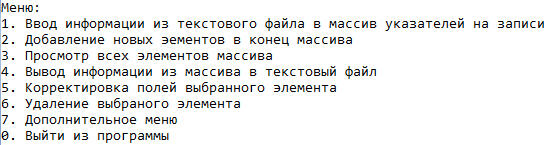
\includegraphics[width=14cm]{_input/programmDevelopment/menu.png}
    \end{center}
    \caption{Организация меню \label{fig:menu}}
\end{figure}

void menu(struct data* array, int length)

\underline{Входные параметры}:

\begin{enumerate}
    \item array- массив типа struct data*
    \item length – размер массива типа int
\end{enumerate}

\underline{Назначение}: организация меню.

\underline{Возвращаемые данные}: пустота.

\hspace{0pt}\\



\textbf{Модуль open\_file}

void open\_file(struct data* array, int length)

\underline{Входные параметры}:

\begin{enumerate}
    \item array- массив типа struct data*
    \item length – размер массива типа int
\end{enumerate}

\underline{Назначение}: попросить размер строки для выделения динамической памяти, попросить строку, для открытия файла, запустить функцию чтения.

\underline{Возвращаемые данные}: пустота.

\hspace{0pt}\\



void read\_file(struct data* array, int length, char* path)

\underline{Входные параметры}:

\begin{enumerate}
    \item array- массив типа struct data*
    \item length – размер массива типа int
    \item path – путь для открытия файла типа char*
\end{enumerate}

\underline{Назначение}: Прочесть файл и отправить данные по полям структуры

\underline{Возвращаемые данные}: пустота.

\hspace{0pt}\\



\textbf{Модуль add\_element\_to\_end}

void add\_element\_to\_end(struct data* array, int length)

\underline{Входные параметры}:

\begin{enumerate}
    \item array- массив типа struct data*
    \item length – размер массива типа int
\end{enumerate}

\underline{Назначение}: Увеличить массив. Запустить функции ввода полей.

\underline{Возвращаемые данные}: пустота.

\hspace{0pt}\\



void input\_name(struct data* array, int length);

void input\_length(struct data* array, int length);

void input\_area(struct data* array, int length);

void input\_number\_of\_ports(struct data* array, int length);

void input\_type(struct data* array, int length);

\underline{Входные параметры}:

\begin{enumerate}
    \item array- массив типа struct data*
    \item length – размер массива типа int
\end{enumerate}

\underline{Назначение}: Ввести данные в поле

\underline{Возвращаемые данные}: пустота.

\hspace{0pt}\\



void view\_all\_elements(struct data* array, int length);

\underline{Входные параметры}:

\begin{enumerate}
    \item array- массив типа struct data*
    \item length – размер массива типа int
\end{enumerate}

\underline{Назначение}: Вывести через цикл все элементы

\underline{Возвращаемые данные}: пустота.

\hspace{0pt}\\



void print\_head\_table();

\underline{Входные параметры}: нет

\underline{Назначение}: напечатать заголовок таблицы

\underline{Возвращаемые данные}: пустота.

\hspace{0pt}\\



void print\_separator();

\underline{Входные параметры}: нет

\underline{Назначение}: напечатать сепартор 

\underline{Возвращаемые данные}: пустота.

\hspace{0pt}\\



void print\_line(int k);

\underline{Входные параметры}:

\begin{enumerate}
    \item k – количество черточек, для подчеркивания таблицы типа int
\end{enumerate}

\underline{Назначение}: напечатать сепартор 

\underline{Возвращаемые данные}: пустота.

\hspace{0pt}\\



\textbf{Модуль save\_to\_tsv\_file}

void save\_to\_tsv\_file(struct data* array, int length);

\underline{Входные параметры}: 

\begin{enumerate}
    \item array- массив типа struct data*
    \item length – размер массива типа int
\end{enumerate}

\underline{Назначение}: записать в файл данные 

\underline{Возвращаемые данные}: пустота.

\hspace{0pt}\\



void fprint\_separator(FILE* file\_pointer);

\underline{Входные параметры}: 

\begin{enumerate}
    \item file\_pointer – указатель на файл типа FILE*
\end{enumerate}

\underline{Назначение}: напечатать в файл сепаратор

\underline{Возвращаемые данные}: пустота.

\hspace{0pt}\\



\textbf{Модуль correct\_field}

void correct\_field(struct data* array, int length);

\underline{Входные параметры}: 

\begin{enumerate}
    \item array- массив типа struct data*
    \item length – размер массива типа int
\end{enumerate}

\underline{Назначение}: вызвать функции корректировки полей 

\underline{Возвращаемые данные}: пустота.

\begin{figure}[!hp]
    \begin{center}
        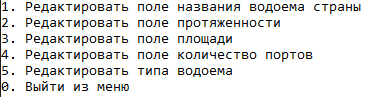
\includegraphics[width=14cm]{_input/programmDevelopment/correctFieldMenu.png}
    \end{center}
    \caption{Организация меню редактирования\label{fig:menu}}
\end{figure}

\hspace{0pt}\\



void correct\_field\_menu(struct data* array, int position);

void correct\_name(struct data* array, int position);

void correct\_length(struct data* array, int position);

void correct\_area(struct data* array, int position);

void correct\_number\_of\_ports(struct data* array, int position);

void correct\_type(struct data* array, int position);

\underline{Входные параметры}: 

\begin{enumerate}
    \item array- массив типа struct data*
    \item length – размер массива типа int
\end{enumerate}

\underline{Назначение}: изменить поле 

\underline{Возвращаемые данные}: пустота.

\hspace{0pt}\\



\textbf{Модуль delete\_element}

void delete\_element(struct data* array, int length);

\underline{Входные параметры}: 

\begin{enumerate}
    \item array- массив типа struct data*
    \item length – размер массива типа int
\end{enumerate}

\underline{Назначение}: удалить определённое поле 

\underline{Возвращаемые данные}: пустота.

\hspace{0pt}\\



\textbf{Модуль clear\_console}

void clear\_console()

\underline{Входные параметры}: нет

\underline{Назначение}: очистка консоли 

\underline{Возвращаемые данные}: пустота.

\hspace{0pt}\\



\textbf{Модуль getch}

void getch()

\underline{Входные параметры}: нет

\underline{Назначение}: ввод одного символа без нажатия пробела 

\underline{Возвращаемые данные}: пустота.

\hspace{0pt}\\



\textbf{Модуль pause\_console}

void pause\_console()

\underline{Входные параметры}: нет

\underline{Назначение}: отстановка выполнения программы, т. к. попросили нажать пользователя клавишу 

\underline{Возвращаемые данные}: пустота.

\hspace{0pt}\\



\textbf{Модуль submenu}

void submenu()

\underline{Входные параметры}: нет

\underline{Назначение}: вывод подменю 

\underline{Возвращаемые данные}: пустота.

\begin{figure}[!hp]
    \begin{center}
        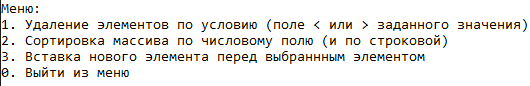
\includegraphics[width=14cm]{_input/programmDevelopment/submenu.png}
    \end{center}
    \caption{Организация подменю\label{fig:submenu}}
\end{figure}

\hspace{0pt}\\



\textbf{Модуль delete\_by\_condition}

void delete\_by\_condition(struct data* array, int length);

\underline{Входные параметры}:

\begin{enumerate}
    \item array- массив типа struct data*
    \item length – размер массива типа int
\end{enumerate}

\underline{Назначение}: вывод меню выбора функции 

\underline{Возвращаемые данные}: пустота.

\hspace{0pt}\\



void delete\_elements\_if\_is\_less\_length(struct data* array, int length);

void delete\_elements\_if\_is\_less\_area(struct data* array, int length);

void delete\_elements\_if\_is\_less\_number\_of\_ports(struct data* array, int length);

void delete\_elements\_if\_is\_more\_length(struct data* array, int length);

void delete\_elements\_if\_is\_more\_area(struct data* array, int length);

void delete\_elements\_if\_is\_more\_number\_of\_ports(struct data* array, int length);

\underline{Входные параметры}:

\begin{enumerate}
    \item array- массив типа struct data*
    \item length – размер массива типа int
\end{enumerate}

\underline{Назначение}: запуск поиска удаления по условию определённого поля 

\underline{Возвращаемые данные}: пустота.

\hspace{0pt}\\



\textbf{Модуль sort\_elementsz}

void sort\_elements(struct data* array, int length);

\underline{Входные параметры}:

\begin{enumerate}
    \item array- массив типа struct data*
    \item length – размер массива типа int
\end{enumerate}

\underline{Назначение}: запуск меню выбора удаления поля 

\underline{Возвращаемые данные}: пустота.

\begin{figure}[!hp]
    \begin{center}
        \includegraphics[width=16cm]{_input/programmDevelopment/sortmenu.png}
    \end{center}
    \caption{Организация меню сортировки\label{fig:sortmenu}}
\end{figure}

\hspace{0pt}\\



void data\_swap(struct data* a, struct data* b);

\underline{Входные параметры}:

\begin{enumerate}
    \item a – один элемент типа struct data* (принимается через адрес \&)
    \item b – второй элемент типа struct data* (принимается через адрес \&)
\end{enumerate}

\underline{Назначение}: обмен двух элементов 

\underline{Возвращаемые данные}: пустота.

\hspace{0pt}\\



void sort\_by\_field\_name(struct data* array, int length);

void sort\_by\_field\_length(struct data* array, int length);

void sort\_by\_field\_area(struct data* array, int length);

void sort\_by\_field\_number\_of\_ports(struct data* array, int length);

void sort\_by\_field\_water\_type(struct data* array, int length);

\underline{Входные параметры}:

\begin{enumerate}
    \item array- массив типа struct data*
    \item length – размер массива типа int
\end{enumerate}

\underline{Назначение}: сортировка по полю 

\underline{Возвращаемые данные}: пустота.

\hspace{0pt}\\



\textbf{Модуль add\_element\_before}

void add\_element\_before(struct data* array, int length);

\underline{Входные параметры}:

\begin{enumerate}
    \item array- массив типа struct data*
    \item length – размер массива типа int
\end{enumerate}

\underline{Назначение}: добавление перед элементом

\underline{Возвращаемые данные}: пустота.
